	\documentclass[11pt]{article}
	\usepackage[utf8]{inputenc}
	\usepackage{listings}
	\usepackage{xcolor}
	\usepackage{float}
	\usepackage{hyperref}
	\hypersetup{breaklinks=true}
	\usepackage{setspace} % Pour gérer l'interligne
	\singlespacing % Définit l'interligne simple
	
	
	\definecolor{dkgreen}{rgb}{0,0.6,0}
	\definecolor{gray}{rgb}{0.5,0.5,0.5}
	\definecolor{mauve}{rgb}{0.58,0,0.82}
	
	\definecolor{eclipseStrings}{RGB}{42,0.0,255}
	\definecolor{eclipseKeywords}{RGB}{127,0,85}
	\colorlet{numb}{magenta!60!black}
	
	\lstdefinelanguage{json}{
		basicstyle=\normalfont\ttfamily,
		commentstyle=\color{eclipseStrings}, % style of comment
		stringstyle=\color{eclipseKeywords}, % style of strings
		numbers=left,
		numberstyle=\scriptsize,
		stepnumber=1,
		numbersep=8pt,
		showstringspaces=false,
		breaklines=true,
		frame=lines,
		backgroundcolor=\color{gray}, %only if you like
		string=[s]{"}{"},
		comment=[l]{:\ "},
		morecomment=[l]{:"},
		literate=
		*{0}{{{\color{numb}0}}}{1}
		{1}{{{\color{numb}1}}}{1}
		{2}{{{\color{numb}2}}}{1}
		{3}{{{\color{numb}3}}}{1}
		{4}{{{\color{numb}4}}}{1}
		{5}{{{\color{numb}5}}}{1}
		{6}{{{\color{numb}6}}}{1}
		{7}{{{\color{numb}7}}}{1}
		{8}{{{\color{numb}8}}}{1}
		{9}{{{\color{numb}9}}}{1}
	}
	\lstset{language=SQL,
		basicstyle={\small\ttfamily},
		belowskip=3mm,
		breakatwhitespace=true,
		breaklines=true,
		classoffset=0,
		columns=flexible,
		commentstyle=\color{dkgreen},
		framexleftmargin=0.25em,
		frameshape={}{yy}{}{}, %To remove to vertical lines on left, set `frameshape={}{}{}{}`
		keywordstyle=\color{blue},
		numbers=none, %If you want line numbers, set `numbers=left`
		numberstyle=\tiny\color{gray},
		showstringspaces=false,
		stringstyle=\color{mauve},
		tabsize=3,
		xleftmargin =1em
	}
	\lstset{
		language=Java,
		basicstyle=\ttfamily\footnotesize,
		keywordstyle=\color{blue}\bfseries,
		stringstyle=\color{red},
		commentstyle=\color{green},
		numbers=left,
		numberstyle=\tiny,
		stepnumber=1,
		numbersep=5pt,
		showspaces=false,
		showstringspaces=false,
		showtabs=false,
		frame=single,
		tabsize=2,
		breaklines=true,
		breakatwhitespace=false,
		escapeinside={\%*}{*)}
	}
	\usepackage{amssymb}
	\usepackage{tabularx}
	\usepackage{longtable}
	\usepackage{pgfplots}
	\pgfplotsset{compat=1.18}
	\usepackage{pgfplotstable}
	\usepackage{graphicx}
	\usepackage{geometry}
	\usepackage{lmodern}
	\usepackage{microtype}
	\usepackage{fancyhdr}
	\usepackage{hyperref}
	\geometry{a4paper, margin=1in}
	
	% en-têtes/pieds de page
	\pagestyle{fancy}
	\fancyhead[L]{Rapport de stage - OPT-NC}
	\fancyhead[R]{Morgan CARRE}
	\fancyfoot[C]{\thepage}
	
	
	\begin{document}
		
		\begin{titlepage}
			\begin{center}
				{\LARGE \textbf{Rapport de Stage}} \\[1cm]
				{\large Effectué du \textbf{02/12/2024} au \textbf{07/02/2025}} \\[1cm]
				
				
				
				{\large Réalisé au sein de la société :} \\[1cm]
				{\Large \textbf{DSI/GLIA OPT-NC}} \\[1cm]
				
				
\includegraphics[width=0.3\textwidth]{asset/logo_opt.jpg} \\[1cm] 
				
				
				\textbf{à Nouméa} \\[1cm]
				
				{\large \textbf{Développement d'une API REST des forfaits télécoms conteneurisée}} \\[0.5cm]
				
				{\large Présenté par :} \\[1cm]
				{\LARGE \textbf{Morgan CARRE}} \\[0.3cm]
				Étudiant en Licence Informatique, Semestre 5 \\[0.3cm]
				\textbf{Université de la Nouvelle-Calédonie} \\[0.3cm]
				
				
\includegraphics[width=0.2\textwidth]{asset/logo_universite.jpg} \\[2cm]
				
				{\large Supervisé par : \textbf{Adrien SALES}} \\[0.3cm]
			\end{center}
		\end{titlepage}
		
		\pagenumbering{gobble} 
		\newpage
		\begin{abstract}
			Dans le cadre de mon stage à l'Université de la Nouvelle-Calédonie (UNC), en collaboration avec l'Office des Postes et Télécommunications de Nouvelle-Calédonie (OPT-NC) supervisé par Adrien SALES, j'ai développé une API permettant de centraliser et d'exposer les informations relatives aux forfaits télécoms proposés par l'OPT-NC. L'objectif principal de ce projet était de fournir une API permettant d’accéder facilement aux données des forfaits pour potentiellement l'intégrer dans diverses applications comme un chatbot sur le site de l'OPT qui conseillerait les clients sur le forfait optimale à choisir ou bien un front-end dynamique.
			
			L'API a été construite à l'aide du framework Quarkus, avec une gestion des migrations de base de données via Flyway. Des outils comme OpenAPI ont été utilisés pour la documentation automatique, tandis que Microcks a permis de simuler les réponses de l'API pour les tests, avant son déploiement réel. La solution a également été conteneurisée grâce à jib, ce qui a simplifié sa gestion et son déploiement. 
			
			Ce rapport détaille les étapes du développement de l'API, les outils utilisés et les solutions mises en œuvre pour permettre une DEVEX (Developer Experience) optimales de l’API.
		\end{abstract}
	
		\newpage
		\section*{Remerciements}
		
		Je tiens à exprimer mes remerciements à toutes les personnes qui ont contribué à la réussite de ce stage et à l’élaboration de ce rapport.
		
		Tout d’abord, je remercie \textbf{Adrien SALES}, mon maître de stage, pour son accompagnement, sa disponibilité et ses conseils précieux tout au long de ce stage. Son expertise et ses retours constructifs ont grandement enrichi mon apprentissage.
		
		Je souhaite également remercier \textbf{Michèle BARRÉ}, pour son aide et l'accompagnement qu'elle m'a apporté tout au long de mon stage.
		
		Je tiens à exprimer ma reconnaissance à toute l’équipe du \textbf{GLIA}, dont \textbf{Adrien SALES}, \textbf{Michèle BARRE}, \textbf{Vinh Faucher}, \textbf{Laurent SCHAEFFER}, \textbf{Romain PELIZZO} et \textbf{Pipiena LUAKI}, pour la bonne ambiance et leur aide, qui ont largement contribué à rendre ce stage agréable et stimulant.
		
		Je remercie enfin \textbf{M. Salmon} d’avoir accepté d’être mon enseignant référent pour ce stage.
	
		\newpage
		\tableofcontents
		\newpage
		\pagenumbering{arabic}
		\section{Introduction}
		
		\subsection{Annonce du stage}
		
		Du \textbf{02 décembre 2024} au \textbf{07 février 2025}, j’ai effectué un stage au sein de l’entreprise \textbf{OPT} (située à Nouméa, Nouvelle-Calédonie). Au cours de ce stage au département \textbf{DSI/GLIA (Direction des Systèmes d'Information / Génie Logiciel Inter-Applicatif)}, j’ai eu l’occasion de me plonger dans le développement d’une API permettant de fournir des informations sur les différents forfaits télécoms proposés par l’entreprise.
		
		Ce stage a été pour moi une opportunité d’explorer plusieurs aspects clés du métier de développeur \textbf{backend}, notamment en matière de gestion de bases de données, d’architecture de microservices cloud natifs, et de l’utilisation des technologies modernes comme Quarkus et Flyway. J’ai également pu développer des compétences techniques liées a la conception d’APIs REST.
		
		\subsection{Bref descriptif de l’entreprise et du déroulement du stage}
		
		L’Office des Postes et Télécommunications de Nouvelle-Calédonie (\textbf{OPT-NC}) est un acteur incontournable en Nouvelle-Calédonie, couvrant un large éventail de secteurs d'activité : intervenant dans les domaines des télécommunications, de la finance, la distribution et des services postaux.
		
		Au sein de son département \textbf{DSI/GLIA}, j’ai intégré une équipe dynamique spécialisée dans le développement, la gestion et l'intégration de solutions logicielles.
		
		
		Supervisé par \textbf{Adrien SALES}, manager de l’équipe \textbf{GLIA}, j’ai bénéficié d’un encadrement rigoureux, favorisant l’apprentissage et la réalisation des différentes missions. Parmi ces missions, j’ai été chargé de concevoir une architecture basée sur Quarkus et Flyway, tout en suivant les bonnes pratiques de développement logiciel.
		
		\subsection{Problématique et objectifs du rapport}
		
		Ce stage m’a permis de développer une API destinée à centraliser et rendre accessibles les informations sur les forfaits télécoms proposés par l’OPT-NC. L’objectif principal était de créer un service, facilitant l’accès à ces données et leur utilisation dans d’éventuelles applications ou analyses.
		
		Ce rapport se concentre sur le processus de développement de l’API, en détaillant les étapes de conception, les choix technologiques réalisés, ainsi que les difficultés techniques rencontrées et les solutions mises en œuvre.
		
		\newpage
		\section{Méthodologie et outils}
		
		\subsection{Méthodologie de travail}
		
		Durant ce stage, j'ai suivi une approche de travail itératif, divisant le développement de l'API en plusieurs tâches spécifiques (appelées \textit{issues}). Chaque tâche correspondait à une fonctionnalité ou une étape précise du projet.
		
		Une fois une tâche terminée, je soumettais mon travail pour vérification à travers une demande spécifique appelée \textit{Pull Request}. Mon maître de stage, Adrien SALES, effectuer les revues de code, identifiait d'éventuelles améliorations ou corrections, et me fournissait des retours. Après validation, les modifications étaient intégrées à la branche \textbf{main}(principale) de la repository, garantissant ainsi une progression structurée et contrôlée.
		
		Des extraits de code sont inclus dans ce rapport, mais le code complet est pour l'instant disponible en Open Source sur le dépôt \textbf{GitHub} à l'adresse suivante : \url{https://github.com/adriens/api-forfaits-opt}.
		
		\subsection{Stack}
		
		Voici les principaux outils et technologies que j’ai utilisés pour ce projet :
	\begin{itemize}
		\item \textbf{Ubuntu} : Système d'exploitation Linux utilisé comme environnement de développement pour le projet.
		\item \textbf{Java} : Langage de programmation principal utilisé pour le développement de l'API.
		\item \textbf{(Apache) Maven} : Outil de gestion des dépendances et d'automatisation de projets java.
		\item \textbf{Quarkus} : Framework Java pour le développement de microservices performants.
		\item \textbf{Flyway} : Outil de gestion des migrations de base de données, assurant la cohérence du schéma de données.
		\item \textbf{H2 Database} : Base de données embarquée utilisée pour les phases de développement et de test.
		\item \textbf{Git et GitHub.com} : Pour la gestion des versions et la collaboration.
		\item \textbf{Visual Studio Code} : Environnement de développement intégré.
		\item \textbf{HTTPie} : Outil en ligne de commande pour tester les endpoints de l'API.
		\item \textbf{Podman} : Outil pour la gestion et l'exécution de conteneurs, utilisé pour tester l'API en environnement conteneurisé.
		\item \textbf{Redocly} : Outil utilisé pour générer de la documentation statique à partir des spécifications OpenAPI.
		\item\textbf{Bump.sh} : Service cloud similaire a Redocly dédié à l'historisation des documentations d'API
		\item \textbf{Jib} : Outil intégré à Maven pour créer des images conteneurisées sans utiliser de \texttt{Dockerfile}. Il simplifie la conteneurisation et génère des images légères et optimisées.
		\item \textbf{SonarQube(.sonarsource.com)} : Outil d'analyse de la qualité du code qui détecte les problèmes, les vulnérabilités et les redondances, améliorant ainsi la qualité et la sécurité du code.
	\end{itemize}
		
		\section{Première tâche : conversion des sous-tâches en issues}
		
		La première tâche qui m’a été confiée était de convertir une liste de sous-tâches fournies par mon maître de stage, Adrien SALES, en \textit{issues} distinctes sur \textbf{Github}. Cette démarche avait pour but de structurer et d’organiser les différentes étapes nécessaires à la réalisation de l’endpoint \texttt{/offres}, qui devait permettre de lister les types de forfaits, leurs pages de référence et une description associée.
		
		\paragraph{Contexte : }
		
		L’issue principale intitulée \textit{/offres : Lister les types d'abonnements \#1} décrivait les objectifs généraux et les actions attendues pour atteindre ce résultat. Voici quelques exemples de sous-tâches qui devaient être transformées en issues individuelles :
		
		\begin{itemize}
			\item Implémenter l'endpoint \texttt{/offres} en injectant les données avec Flyway
			\item Documenter avec des spécifications OpenAPI complètes
			\item Ajouter une CI pour tester le build Maven
			\item Générer une documentation HTML statique avec Redocly
		\end{itemize}
		\begin{center}
			\textbf{Exemple d'issue mise en forme :}
		\end{center}
		\begin{center}
			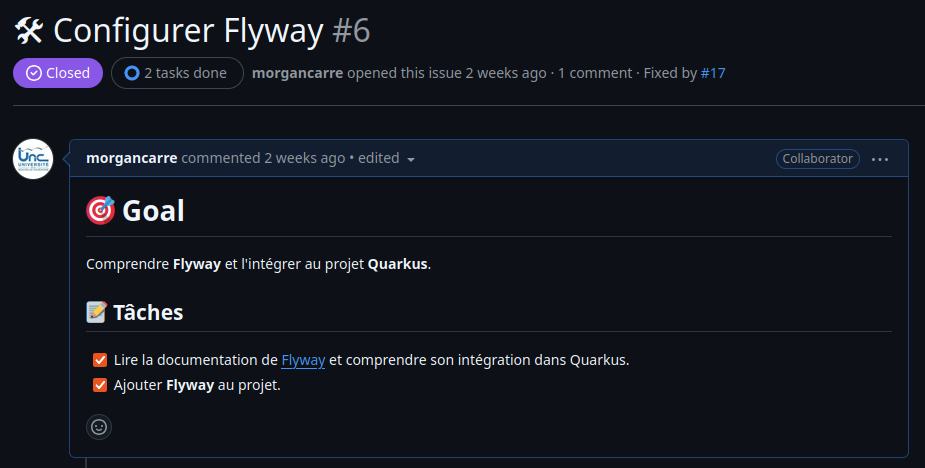
\includegraphics[width=0.8\textwidth]{asset/ex_issue.png}
		\end{center}
		
		Ce format inclut le titre de l’issue, une description détaillée des objectifs, et parfois des liens vers des ressources ou des outils nécessaires à sa réalisation.
		
		 Cette structuration a permis une meilleure visibilité sur les étapes du projet, tout en facilitant le suivi et la validation des différentes phases par mon maître de stage.
		\section{Identification des types de forfaits et création du fichier \texttt{offres.csv}}
		
		Ma deuxième tâche a consisté à identifier les différents types de forfaits disponibles sur la page de l’OPT intitulée \textit{"Identifiez le forfait qui vous ressemble"} (voir Figure~\ref{fig:page_forfait} dans l'Annexe). Pour cela, j’ai analysé les caractéristiques propres à chaque forfait, notamment leur nom, leur description et leur utilisation, afin de les préparer sous une forme exploitable.
		
		\subsection*{Structuration dans un fichier \texttt{CSV}}
		Après cette analyse, j’ai structuré ces informations dans un fichier au format \texttt{CSV}, nommé \texttt{offres.csv}. Ce fichier contient les champs suivants : l’identifiant (\texttt{id}), le nom (\texttt{desc}) et la description détaillée (\texttt{desc full}) de chaque forfait.
		
		J’ai choisi le format \texttt{CSV} en raison de sa portabilité et de sa facilité d’exploitation dans de nombreux cas. Ce format est particulièrement adapté à notre contexte, car il permet de charger efficacement les données dans une base de données à l’aide de Flyway, un outil utilisé pour gérer les migrations et remplir les tables avec les données préparées.
		
		\section{Initialisation du projet Quarkus et création d’un endpoint \textit{Hello World}}
		
		Une des premières étapes de mon projet a été d’initialiser le projet Quarkus et de mettre en place un endpoint basique permettant de tester le bon fonctionnement de l’environnement.
		
		\subsection{Initialisation du projet Quarkus}
		
		Pour initialiser le projet, j’ai utilisé la commande suivante :
		\begin{verbatim}
			mvn io.quarkus:quarkus-maven-plugin:create
		\end{verbatim}
		
		Cette commande a automatiquement généré la structure de base du projet, comprenant plusieurs fichiers et répertoires essentiels. Parmi les éléments les plus importants, on trouve :
		\begin{itemize}
			\item \texttt{pom.xml} : le fichier de configuration Maven qui liste les dépendances nécessaires au projet.
			\item \texttt{src/main/java} : le répertoire contenant le code source de l’application, avec un premier exemple de classe.
			\item \texttt{src/main/resources} : le répertoire pour les fichiers de configuration et les ressources statiques, comme notre fichier \textbf{CSV}.
			\item \texttt{src/test/java} : le répertoire dédié aux tests unitaires.
		\end{itemize}
		
		Par défaut, Quarkus inclut un endpoint basique accessible à l’adresse \texttt{/hello}, qui renvoie un simple message \textit{"Hello World"}.
		
		\subsection{Lancement et test du projet}
		
		Pour exécuter le projet, il suffit d’utiliser la commande suivante :
		\begin{verbatim}
			mvn quarkus:dev
		\end{verbatim}
		
		Cette commande lance le projet en mode développement, avec un support pour le \textit{live coding}. Cela signifie que toutes les modifications apportées au code ou aux fichiers de configuration sont appliquées instantanément, sans besoin de redémarrer le serveur.
		
		Une fois lancé, le projet est accessible en local à l’adresse suivante :
		\begin{verbatim}
			http://localhost:8080
		\end{verbatim}
		
		J’ai ensuite vérifié le bon fonctionnement de l’endpoint par défaut \texttt{/hello} grâce à un appel réalisé avec l’outil HTTPIE (Voir figure \ref{fig:hello_endpoint} dans l'annexe).
		
		\subsection{Avantages de Quarkus pour le développement}
		
		L’utilisation de Quarkus offre plusieurs avantages, notamment :
		\begin{itemize}
			\item Une structure de projet standardisée et prête à l’emploi, permettant de se concentrer rapidement sur le développement des fonctionnalités.
			\item Une DevEx optimale via un mode de développement interactif grâce à \textit{mvn quarkus:dev}, qui améliore la productivité.
			\item La possibilité d’ajouter facilement des extensions pour enrichir le projet, telles que Flyway ou Hibernate.
			\item Un \textit{Dev UI}, une interface graphique intégrée qui facilite le développement en permettant de visualiser et d'interagir avec l'application en temps réel. Cela permet de tester et de déboguer plus rapidement sans avoir à effectuer de nombreuses actions manuelles.
		\end{itemize}
		
		Cette première étape m’a permis de comprendre l’organisation d’un projet Quarkus et de mettre en place un environnement fonctionnel prêt à accueillir des fonctionnalités plus avancées.
		
		\section{Configuration de Flyway et mise en place de l'endpoint \texttt{/offres}}
		
		Dans le cadre de ce projet, il était nécessaire de centraliser les données des forfaits télécoms dans une base de données et de les exposer via un endpoint accessible. Pour ce faire, j'ai configuré Flyway pour gérer la base de données et j'ai développé l'endpoint \texttt{/offres} permettant de récupérer ces données.
		
		\subsection{Configuration de Flyway et de la base de données H2}
		
		La gestion de la base de données a été confiée à Flyway, une solution reconnue pour son efficacité et sa simplicité d'intégration dans des projets modernes. Voici les principales étapes de configuration :
		
		\begin{itemize}
			\item Ajout des dépendances nécessaires dans le fichier \texttt{pom.xml} :
			\begin{itemize}
				\item \texttt{quarkus-flyway} : pour gérer les migrations de la base de données.
				\item \texttt{quarkus-jdbc-h2} : pour utiliser une base de données H2 en mémoire.
				\item \texttt{quarkus-hibernate-orm} : pour mapper les entités avec les tables de la base de données.
				\item \texttt{quarkus-rest-jackson} : pour gérer les réponses JSON dans les endpoints REST.
			\end{itemize}
			
			\item Configuration dans le fichier \texttt{application.properties}
			définissant une base de données en mémoire H2, qui est initialisée à chaque démarrage de l'application et remplie  automatiquement grâce à Flyway.
			
			\item Création du fichier de migration \texttt{V1\_\_create\_and\_feed\_forfaits.sql} :
			Ce fichier SQL configure la table \texttt{forfaits} et y insère les données issues du fichier \texttt{offres.csv} grâce à la méthode \texttt{CSVREAD}.
		\end{itemize}
		
		\subsection{Mise en place de l'endpoint \texttt{/offres}}
		
		L'endpoint \texttt{/offres} a été conçu pour exposer les données des forfaits télécoms sous forme JSON. Voici les étapes principales de son implémentation :
		\subsection*{Création de l'entité \texttt{Forfait}}
		\begin{itemize}
			\item Création de l'entité \texttt{Forfait}, mappée avec la table \texttt{forfaits} dans la base de données. Cette classe représente la table \texttt{forfaits} dans la base de données. 	
			
			\begin{itemize}
				\item
				\begin{lstlisting}
					@Entity
					@Table(name = "forfaits")
					public class Forfait {
					\end{lstlisting}
					\begin{itemize}
						\item L'annotation \texttt{@Entity} indique que cette classe est une entité JPA, mappée sur une table dans la base de données.
						\item L'annotation \texttt{@Table(name = "forfaits")} spécifie le nom de la table associée à cette entité.
					\end{itemize}
					
					\item
					\begin{lstlisting}
						@Id
						private String id;
					\end{lstlisting}
					\begin{itemize}
						\item L'annotation \texttt{@Id} désigne le champ \texttt{id} comme étant la clé primaire de la table \texttt{forfaits}.
					\end{itemize}
					
					\item
					\begin{lstlisting}
						private String desc;
						private String description;
					\end{lstlisting}
					\begin{itemize}
						\item Ces champs représentent les colonnes \texttt{desc} et \texttt{description} dans la table \texttt{forfaits}.
					\end{itemize}
			\end{itemize}
		\end{itemize}
				
			
			Cette classe joue un rôle crucial, car elle permet de manipuler les données de la table \texttt{forfaits} comme des objets Java.
		\subsection*{Développement de la ressource REST \texttt{OffresResource}}
		
		\begin{itemize}
			\item \begin{lstlisting}
				@Path("/offres")
				@Produces(MediaType.APPLICATION_JSON)
				public class OffresResource {
				\end{lstlisting}
				\item L'annotation \texttt{@Path("/offres")} définit l'endpoint \texttt{/offres}.
				\item L'annotation \texttt{@Produces(MediaType.APPLICATION\_JSON)} indique que la réponse sera au format JSON.
				
				\item \begin{lstlisting}
					@GET
					public List<Forfait> getAllOffres() {
						return entityManager.createQuery("SELECT f FROM Forfait f", Forfait.class).getResultList();
					}
				\end{lstlisting}
				\item La méthode \texttt{getAllOffres()} est mappée à la méthode HTTP \texttt{GET} et renvoie tous les enregistrements de la table \texttt{Forfait}.
			\end{itemize}
	
		\subsection*{Validation de l'endpoint avec HTTPIE}
		
		Pour vérifier le bon fonctionnement de l'endpoint \texttt{/offres}, un appel a été effectué à l'aide de l'outil HTTPIE (Voir Figure \ref{fig:offres_endpoint} dans l'annexe).
		
		\section{Conteneurisation de l'API}
		
		\subsection*{Pourquoi conteneuriser ?}
		
		La conteneurisation permet d'encapsuler une application, ses dépendances et son runtime complet ce qui en permet un déploiment aisé par tout un chacun. Ce conteneur peut être exécuté de manière identique sur différentes machines, ce qui assure sa portabilité.
		
		\subsection*{Solution proposée : JIB}
		
		Mon tuteur m'a conseillé d'utiliser \textbf{JIB}, un outil de conteneurisation intégré à Maven. JIB permet de construire une image optimisée sans \texttt{Dockerfile}, en exploitant directement les ressources nécessaires identifiées par Maven.
		
		\subsection*{Configuration de JIB}
		
		J'ai configuré JIB dans le projet en suivant ces étapes :
		\begin{enumerate}
			\item \textbf{Ajout de la dépendance dans \texttt{pom.xml}}
			\item \textbf{Configuration dans \texttt{application.properties}} :	
			
			\begin{itemize}
				\item \texttt{quarkus.container-image.build=true} : Active la fonctionnalité de génération d'image conteneurisée lors de la construction du projet.
				\item \texttt{quarkus.jib.docker-executable-name=podman} : Indique à Jib d'utiliser Podman comme runtime de conteneur. Podman est une alternative à Docker, légère et adaptée aux environnements rootless (sans besoin de privilèges root).
				\item \texttt{quarkus.jib.base-jvm-image=openjdk:23-jdk} : Spécifie l'image de base utilisée pour l'image conteneurisée. Dans ce cas, l'image \texttt{openjdk:23-jdk} Spécifie la version Java à utiliser, ici Java 23 (par défaut java 21).
				\item \texttt{quarkus.container-image.name=forfaits-opt-nc} : Définit le nom de l'image.
			\end{itemize}
	
			Cette configuration permet d'automatiser la création d'une image conteneurisée avec Jib.
			\item \textbf{Commandes pour builder et exécuter l'image} :
			\begin{itemize}
				\item \textbf{Construction de l'image} :
				\begin{verbatim}
					mvn package
				\end{verbatim}
				\item \textbf{Lancement du conteneur} :
				\begin{verbatim}
					podman run --name forfaits-container\
					-p 8080:8080\
					forfaits-opt-nc:1.0.0-SNAPSHOT
				\end{verbatim}
			\end{itemize}
		\end{enumerate}
		\subsection*{Validation de l'approche}
		
		Pour valider la conteneurisation, j'ai utilisé Podman Desktop pour vérifier que l'image a bien été générée. Ensuite, j'ai testé l'API en exécutant une requête HTTPie sur l'endpoint \texttt{/offres}. Voici les résultats obtenus :
		\begin{itemize}
			\item \textbf{Après le build de l'image avec \texttt{mvn package}} : La capture d'écran montre l'image générée dans Podman Desktop.
			\begin{figure}[h!]
				\centering
				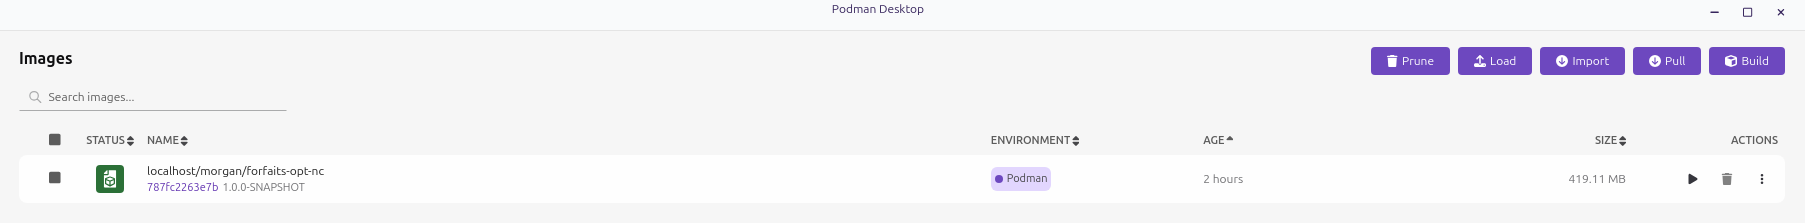
\includegraphics[width=1\textwidth]{asset/image_podman.png}
				\caption{Capture d'écran de l'image générée dans Podman Desktop.}
				\label{fig:image_podman}
			\end{figure}
			
			\item \textbf{Après l'exécution de l'image avec \texttt{podman run}} : L'exécution de l'image crée un conteneur, vérifiable via Podman Desktop. Une capture d'écran du conteneur en cours d'exécution est ajoutée pour valider cette étape.
			\begin{figure}[h!]
				\centering
				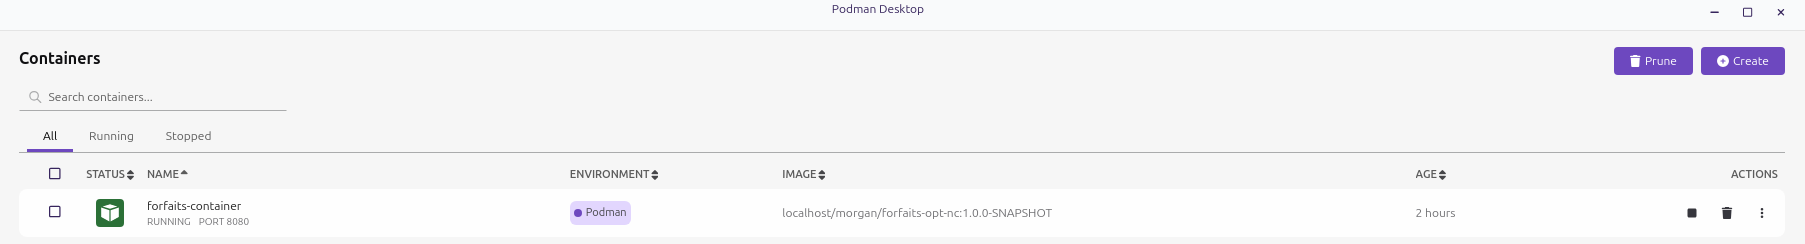
\includegraphics[width=1\textwidth]{asset/conteneur_podman.png}
				\caption{Capture d'écran du conteneur en cours d'exécution dans Podman Desktop.}
				\label{fig:conteneur_podman}
			\end{figure}
		\end{itemize}
		\subsection*{Amélioration de l'expérience développeur}
		
		Mon tuteur a également souligné l'importance de la Developer Experience (\textbf{DevEx}). Grâce à JIB, la génération des conteneurs est simplifiée, rapide et reproductible, ce qui réduit considérablement les efforts nécessaires pour maintenir et déployer l'API.
		
		\section{Documentation de l'API}
		
		La documentation d'une API est essentielle pour garantir une utilisation efficace et correcte de celle-ci par les developpeurs désireux de la consommer. Elle facilite la compréhension des fonctionnalités offertes, les méthodes disponibles, les formats de données acceptés, et les réponses possibles. Une API bien documentée améliore non seulement la DevEx mais aussi la maintenance et l'évolution du service.
		
		\subsection{Utilisation de OpenAPI}
		
		Dans ce projet, la spécification \textbf{OpenAPI} a été choisi pour documenter automatiquement l'API. Grâce à elle, la documentation est générée directement à partir des annotations. Cela permet d'avoir une documentation de l'API toujours à jour. 
		
		L'intérêt principal d'OpenAPI est sa capacité à produire une spécification au format \texttt{YAML} et \texttt{JSON}, qui pourra être utilisée par la suite par exemple pour générer du code client (js, node, Python, Go,...).
		
		La configuration de OpenAPI dans le projet a été réalisée avec les étapes suivantes :
		\begin{itemize}
			\item Ajout de la dépendance \texttt{quarkus-smallrye-openapi} dans le fichier \texttt{pom.xml}.
			\item Annotation des endpoints pour décrire leur fonctionnement et leurs objectifs:
		\end{itemize}
			
		\begin{itemize}
			\item \texttt{@Path("/offres")} : Ajoute l'URL de l'endpoint \texttt{/offres}.
			\item \texttt{@Produces(MediaType.APPLICATION\_JSON)} : Indique que la réponse de cet endpoint sera au format JSON.
			\item \texttt{@GET} : Indique que cet endpoint utilise la méthode HTTP GET pour récupérer des données.
			\item \texttt{@Tag} : Ajoute une catégorie (\texttt{Forfaits}) et une description détaillant la fonctionnalité de l'endpoint ("Liste les différentes gammes d'offres télécoms de l'OPT").
			\item \texttt{@Operation} : Décrit l'opération spécifique de l'endpoint, permettant de préciser son but et son fonctionnement dans la documentation OpenAPI. \item \texttt{@APIResponses} : Permet de spécifier les différentes réponses possibles d'un endpoint, en indiquant notamment les codes de statut HTTP associés et leur signification. 
		\end{itemize}
	
		\subsection{Utilisation de Redocly pour la génération de documentation HTML statique}
		\label{subsec:redocly}
		
		Dans ce projet, l'outil \textbf{Redocly} a été utilisé pour générer une documentation HTML statique de l'API à partir des spécifications OpenAPI générées précédemment. La documentation produite est une interface graphique interactive, permettant aux utilisateurs de mieux comprendre les fonctionnalités de l'API.
		
		\subsection{Mise en place d'un workflow GitHub Actions}
		
		Pour automatiser la génération de la documentation à chaque nouvelle release, un workflow \textbf{GitHub Actions} a été intégré dans le projet. Ce workflow est déclenché automatiquement dès qu'une nouvelle release est publiée sur GitHub, et il permet de générer la documentation statique à l'aide de Redocly, puis de la déployer directement sur \textbf{GitHub Pages}.
		
		Voici les étapes principales de ce workflow :
		\begin{itemize}
			\item \textbf{Installation de Node.js} : Le workflow commence par l'installation de \texttt{Node.js} via l'action \texttt{actions/setup-node@v3}. Node.js est nécessaire pour exécuter Redocly.
			\item \textbf{Installation de Redocly} : Ensuite, Redocly est installé à l'aide de la commande \texttt{npm i -g @redocly/cli@latest}.
			\item \textbf{Génération de la documentation HTML} : Le workflow génère la documentation statique (Voir la figure \ref{fig:html_redocly} dans l'annexe) en exécutant \texttt{redocly build-docs}, qui prend le fichier OpenAPI (\texttt{openapi.yaml}) et génère une page HTML dans le répertoire \texttt{./docs}.
			\item \textbf{Déploiement sur GitHub Pages} : Enfin, la documentation est déployée sur GitHub Pages en utilisant l'action \texttt{actions/deploy-pages@main}.
		\end{itemize}
		
		Cette approche permet non seulement de maintenir la documentation à jour automatiquement, mais aussi de l'héberger de manière simple et accessible via GitHub Pages à l'url : \url{https://adriens.github.io/api-forfaits-opt/}.
		
		\section{bump.sh et Redocly : Comparaison et Mise en Place}
		
		\textbf{bump.sh} est une plateforme qui facilite la gestion, la publication et l'historisation de la documentation d’API, avec une fonctionnalité unique de suivi des différences détaillant les ajouts et modifications entre les versions de l'API. Contrairement à \textbf{Redocly}, qui génère uniquement la documentation.
		\begin{table}[h!]
			\centering
			\begin{tabularx}{\textwidth}{|X|X|X|}
				\hline
				\textbf{Critère} & \textbf{Bump.sh} & \textbf{Redocly} \\
				\hline
				\textbf{Génération de la documentation} & $\checkmark$ & $\checkmark$ \\
				\hline
				\textbf{Suivi des versions} & $\checkmark$ & $\times$ \\
				\hline
				\textbf{Prise en charge de l'intégration CI/CD} & $\checkmark$ & $\checkmark$ \\
				\hline
				\textbf{Support pour les APIs} &  \textbf{OpenAPI},\textbf{AsyncAPI}, \textbf{GraphQL}, \textbf{gRPC}, \textbf{SOAP} & \textbf{OpenAPI} \\
				\hline
				\textbf{Mise à jour automatique de la documentation} & $\checkmark$ & $\checkmark$ \\
				\hline
			\end{tabularx}
			\caption{Comparaison entre Bump.sh et Redocly}
		\end{table}
		\subsection*{Mise en place de Bump.sh}
		
		Pour mettre en place Bump.sh dans ce projet, j'ai procédé à l'upload d'une spécification OpenAPI au format YAML sur la plateforme Bump.sh. Voici les étapes réalisées :
		
		\begin{itemize}
			\item J'ai récupéré le fichier de spécification OpenAPI au format \textbf{openapi.yml} généré lors du build.
			\item J'ai téléchargé ce fichier sur la plateforme Bump.sh, qui a automatiquement généré la documentation de l'API (Voir la figure \ref{fig:bumpsh}).
			\item Bump.sh l'a hébergée en ligne pour un accès facile et publique à l'url \url{https://bump.sh/morgancarre/doc/forfaits-opt-nc}.
		\end{itemize}
			
		\section{Mise en place des tests unitaires et de la couverture de code}
		\label{subsec:test-offres}
		Les tests unitaires permettent de valider le bon fonctionnement des différentes parties du code.
		Afin de garantir la qualité du code et de s'assurer que les tests couvrent suffisamment les différentes parties de l'application, nous avons mis en place des tests unitaires accompagnés d'une vérification de la couverture de code avec un seuil minimum de 10\%. 
		Pour ce projet, nous avons utilisé \texttt{JUnit} en combinaison avec \texttt{QuarkusTest}, une extension de Quarkus permettant de tester les endpoints, ainsi que JaCoCo pour mesurer le taux de couverture du code. 
		
		\subsection{Test de l'endpoint \texttt{/offres}}
		
	
			\begin{lstlisting}[language=Java]
					@Test
					public void testGetAllOffres() {
						given().when().get("/offres")
						.then().statusCode(200)
						.body("$", hasSize(5));
					}
			\end{lstlisting}
				Le test \texttt{testGetAllOffres} vérifie que l'endpoint \texttt{/offres} répond avec un code HTTP 200 et contient bien 5 offres.
	
		
		\subsection{Ajout de la dépendance JaCoCo}
		Pour mesurer la couverture des tests unitaires, nous avons utilisé \textbf{JaCoCo}, un outil de couverture de code Java. JaCoCo génère un rapport indiquant la proportion de code exécutée par les tests, ce qui permet d'identifier les parties du code qui ne sont pas couvertes.
		
		La dépendance JaCoCo a été ajoutée dans le fichier \texttt{pom.xml} puis le plugin \texttt{jacoco-maven-plugin} a été configuré pour mesurer la couverture de code et générer un rapport détaillé après l'exécution des tests.
		
		Dans cette configuration, le seuil de couverture est fixé à 10\%, ce qui signifie que si moins de 10\% des lignes de code sont couvertes par les tests, le build échouera.
		
		\begin{figure}[h!]
			\centering
			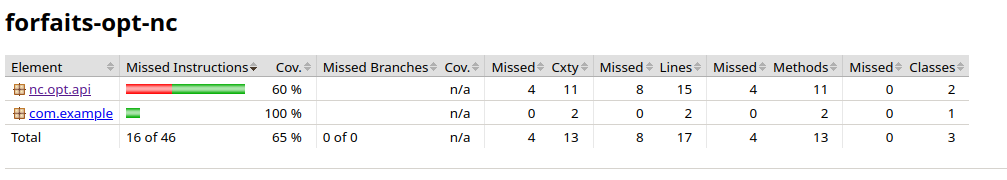
\includegraphics[width=\textwidth]{asset/jacoco.png}
			\caption{Capture d'écran du rapport de couverture généré par JaCoCo}
			\label{fig:jacoco-report}
		\end{figure}
		
		\subsection{Configuration du pipeline CI avec GitHub Actions et SonarQube}
		Pour automatiser l'exécution des tests, la validation du build et l'analyse de la qualité du code, un pipeline CI a été configurée avec \textbf{GitHub Actions}. Ce pipeline s'exécute à chaque push ou pull request sur la branche \texttt{main}.
		
		\subsection{SonarQube}
		SonarQube est un outil de qualité de code qui permet d'analyser en profondeur le code source, d'identifier des problèmes de qualité, des vulnérabilités et des codes redondants. Dans ce projet, SonarQube est intégré au pipeline CI et directement aux Pull Requests (PRs), permettant une analyse automatique et un retour immédiat à chaque soumission. Cette intégration assure une expérience développeur (DevEx) optimale et continue en garantissant une qualité de code constante avant fusion.
		
		Pour l'intégration de SonarQube, voici les étapes réalisées :
		\begin{itemize}
			\item \textbf{Ajout de la configuration dans le fichier \texttt{pom.xml}} : J'ai ajouté la configuration suivante pour lier le projet à SonarQube Cloud :

		
			\item\textbf{Intégration dans la pipeline CI} : inclut l'installation du JDK, la mise en cache des packages Maven et SonarQube, l'exécution des tests et l'analyse SonarQube (exemple d'analyse : \ref{analyse:sonar}).
		\end{itemize}
		\section{Nouvel endpoint : /offres/forfait-m}
		L'objectif principal de ce nouvel endpoint est de fournir les différentes offres de la gamme "M", incluant des informations telles que :le nom, le prix,la volumétrie de données (par exemple : 1 Go, 5 Go, 25 Go, 100 Go), le temps d'appel (1h, appels illimités...), les SMS (illimités ou limités), l'url qui redirige sur le site de l'OPT
	
		J'ai donc suivi le même schéma que pour l'endpoint /offres :
		
		\subsection*{Mise en place des données}
		\label{subsec:mpd}
		Je me suis donc rendu sur le site de l'OPT pour récuperer les informations publiquement disponibles sur chaque forfait M pour les mettre en forme dans un fichier \texttt{forfait\_m.csv}
		contenant les 6 champs décrit plus haut : 
		\begin{itemize} 
			\item \textbf{id} (le nom unique du forfait)
			\item \textbf{prix}
			\item \textbf{sms}
			\item \textbf{url}
			\item \textbf{vocal}
			\item \textbf{volumétrie}
		\end{itemize}
		
		Ensuite j'ai créé mon deuxième fichier de migration SQL \texttt{V2\_\_create\_and\_feed\_forfait\_m.sql} que Flyway exécutera au boot de l'application. 
		
		Il créera une table \texttt{forfait\_m} puis remplira cette table avec le fichier \texttt{forfait\_m.csv} : 
		\subsection*{Création de l'entité ForfaitM}
		\label{subsec:JPA}
		Pour pouvoir manipuler la base de donnée en Java,comme pour l'endpoint \texttt{/offres}, il faut créer une entité JPA \texttt{ForfaitM.java} :
		
		On lie la table à notre entité java :
		\begin{lstlisting}[language=java]
			@Entity
			@Table(name = "forfait_m") 
		\end{lstlisting}
		
		On crée notre classe \texttt{ForfaitM} en définissant les paramètres de l'entité et en ajoutant les "getter" pour chaque attribut.
			
		\subsection*{Développement de l'endpoint /offres/forfaits-m}
		\label{subsec:endpoint-m}
		Dans cette section, nous allons implémenter l'endpoint \texttt{/offres/forfaits-m} pour exposer les forfaits de la gamme "M". Cet endpoint comportera deux méthodes principales.
		
		\begin{itemize}
			\item La première méthode, \texttt{GET /offres/forfait-m}, permet de récupérer la liste de tous les forfaits de la gamme "M". 
			Elle utilise l'annotation \texttt{@GET} et la méthode \texttt{createQuery} d'\texttt{EntityManager} pour effectuer une requête JPQL qui sélectionne tous les enregistrements de la table \texttt{ForfaitM}. 
			Le résultat est retourné sous forme d'une liste d'objets \texttt{ForfaitM}.
		\end{itemize}
		
		Voici la requête avec HTTPie : 
		
		\begin{lstlisting}
			http GET :8080/offres/forfait-m
		\end{lstlisting}
		\begin{lstlisting}[language=json]
			[
			{
				"id": "forfait-m-1",
				"prix": 1000.0,
				"sms": "SMS illimites",
				"url": "https://www.opt.nc/particuliers/mobile/quel-forfait-choisir/forfait-m-1-go",
				"vocal": "1H",
				"volumetrie": "1 Go"
			},
				[tous les autres forfait M]...
			]
			
		\end{lstlisting}
		
		\begin{itemize}
			\item La deuxième méthode, \texttt{GET /offres/forfait-m/{id}}, permet de récupérer les détails d'un forfait spécifique, identifié par \texttt{id}. 
			Cette méthode prend un paramètre \texttt{id} extrait de l'URL, grâce à \texttt{@PathParam}, et l'utilise dans une requête JPQL pour chercher un forfait particulier dans la table \texttt{ForfaitM}. 
			La méthode \texttt{getSingleResult} est utilisée pour récupérer un seul enregistrement correspondant à l'identifiant fourni.
		\end{itemize}
		\subsection*{Gestion des erreurs 404 lors de la saisie d'un mauvais ID}
		\label{subsec:error-handling}
		
		Dans le cadre de l'implémentation des endpoints de l'API, il est crucial de gérer correctement les erreurs, en particulier lorsque l'utilisateur fournit des identifiants invalides. La gestion des erreurs permet d'optimiser l'expérience utilisateur, de garantir la sécurité de l'application.
		
		Lorsque l'utilisateur demande des informations sur un forfait en utilisant un identifiant (ID) qui n'existe pas dans la base de données, il est essentiel que l'API réagisse de manière adéquate. Une réponse 404 est une manière standard de signaler que la ressource demandée est introuvable. 
		
		\textbf{Implémentation de l'erreur 404} : 
		Lorsqu'un ID erroné est fourni par l'utilisateur, l'API retourne une réponse 404 ainsi q'un message d'erreur "Forfait avec ID : (id invalide) non trouvé".Pour ce faire, un bloc \texttt{try-catch} est utilisé pour capturer une exception si l'ID fourni n'existe pas dans la base de données.
	
		
		\subsection*{Tests unitaires}
		\label{subsec:tests}
		
		Les tests unitaires sont mis en place avec un seuil de couverture de 10\%. Ils vérifient les comportements suivants :
		
		\begin{itemize}
			\item Le test sur \texttt{/offres/forfait-m} vérifie que l'endpoint renvoie 4 forfaits, avec l'ID du premier à \texttt{"forfait-m-1"}.
			\item Le test sur \texttt{/offres/forfait-m/{id}} vérifie qu'un forfait avec un ID spécifique renvoie correctement les informations, comme le prix.
			\item Le test \texttt{NotFound} pour \texttt{/offres/forfait-m/{id}} vérifie la gestion des erreurs avec un message adapté en cas d'ID inconnu.
		\end{itemize}
	
		\subsection*{Ajout de la documentation}
		\label{subsec:doc}
		
		Comme pour l'endpoint \textbf{/offres} j'ai utilisé les annotations \textbf{openapi} pour documenter cet endpoint.
		
		Voici les nouvelles annotations utilisées:
		
		\begin{itemize}
			\item \textbf{\texttt{@Operation}} : Décrit les actions effectuées par un endpoint (ex. : récupérer un forfait spécifique).
			\item \textbf{\texttt{@Parameter}} : Déclare les paramètres d'entrée d'un endpoint, comme l'ID du forfait à récupérer.
			\item \textbf{\texttt{@APIResponse}} : Définit les réponses possibles d'un endpoint, incluant les codes de réponse et les exemples de données retournées.
			\item \textbf{\texttt{@Tag}} : Permet de regrouper les endpoints sous une même catégorie pour mieux organiser la documentation.
			\item \textbf{\texttt{@ExampleObject}} : Fournit des exemples de réponses pour aider à comprendre le format des données.
		\end{itemize}
		
		En générant la documentation statique avec Redocly à partir de ces annotations OpenAPI, nous avons pu obtenir une documentation claire et bien structurée (voir figure \ref{fig:redocly}).
		
		\subsection*{Analyse avec SonarQube}
		\label{analyse:sonar}
		Une fois les nouvelles fonctionnalités ajoutées, j'ai ouvert une pull request pour fusionner la branche sur laquelle j'ai développé ces fonctionnalités avec la branche principale. Cela a déclenché la CI, incluant les tests unitaires et l'analyse avec SonarQube. SonarQube a ensuite généré un bref résumé de l'analyse dans les commentaires de la pull request : 
		
			\begin{figure}[H] \centering 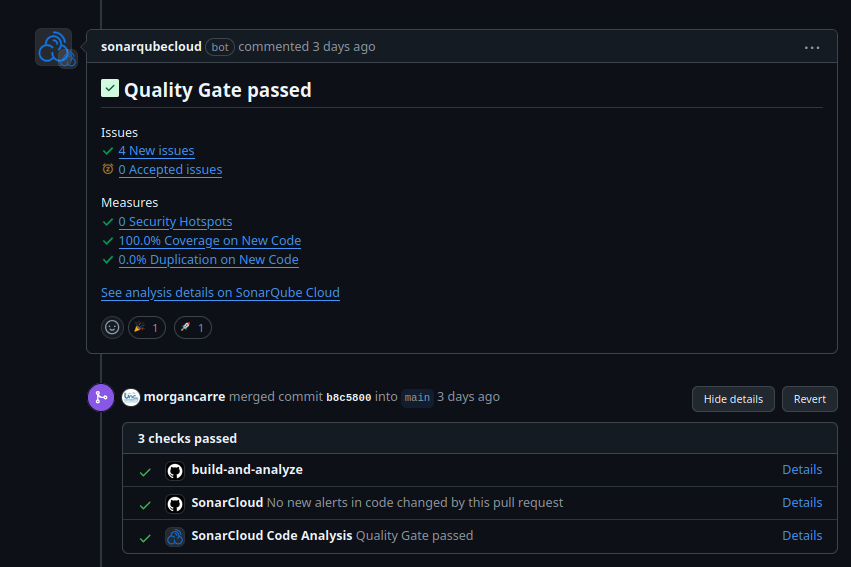
\includegraphics[width=0.7\textwidth]{asset/sonarq_com.png} \caption{commentaire de SonarQube} \label{fig:sonarq}\end{figure}
		
		En cliquant sur le lien "See analysis details on SonarQube cloud" dans son commentaire, nous pouvons accéder aux détails de l'analyse du nouveau code qui a été poussé (voir figure \ref{fig:sonarq} ). 
		
		Cette analyse inclut principalement les informations suivantes : \begin{itemize} \item Le pourcentage de couverture du code par les tests. \item Les éventuelles vulnérabilités et les problèmes de qualité détectés dans le code. \item Les règles de code respectées et celles enfreintes. \item Des suggestions d'amélioration pour optimiser la qualité du code. \end{itemize}
		
		\subsection*{Nouvelle release et delivery  automatique de la documentation}
		
		Une fois la branche fusionnée avec la branche principale, j'ai effectué une nouvelle release. Le workflow pour déployer sur GitHub Pages s'est alors déclenché et a déployé la documentation de l'API à l'adresse \url{https://adriens.github.io/api-forfaits-opt/}. \ J'avais également ajouté un autre workflow pour déployer la documentation automatiquement sur \textbf{Bump.sh}. Celui-ci s'est également déclenché lors de la publication de la release, et j'ai pu consulter le rapport de changement de version.
		\begin{figure}[H] \centering 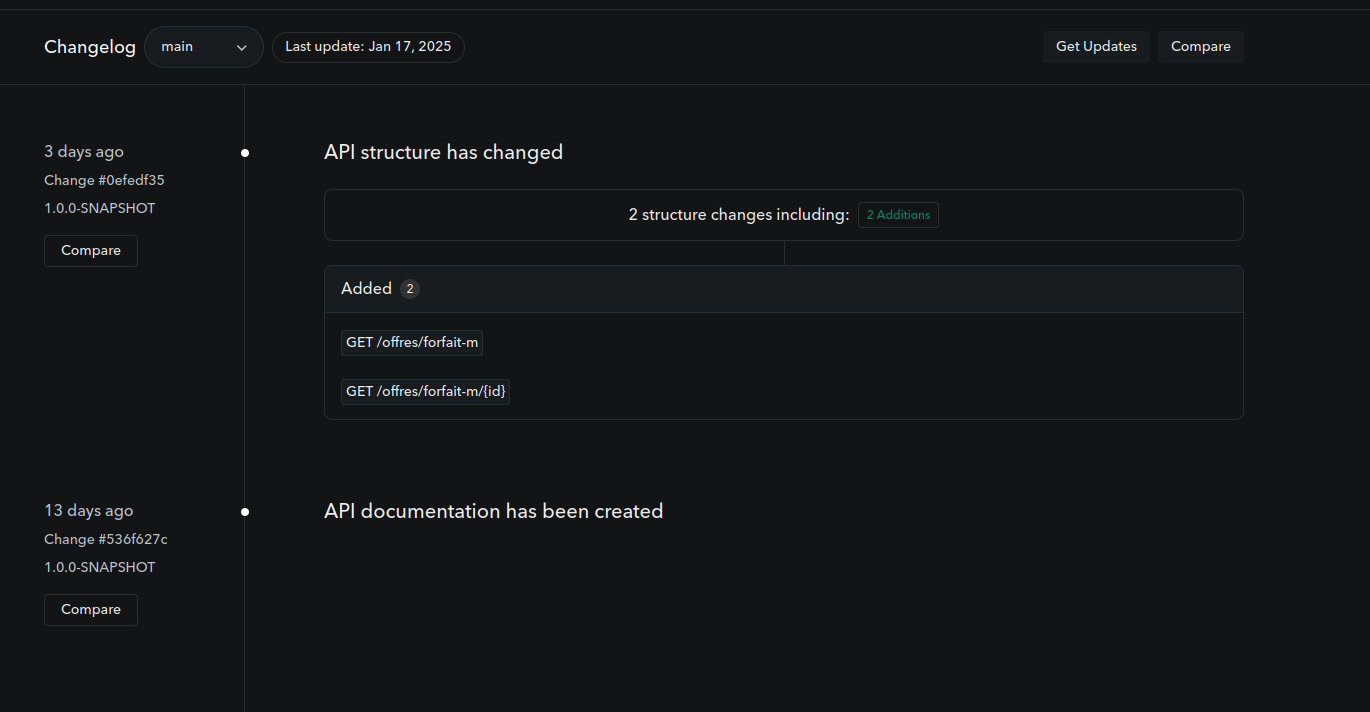
\includegraphics[width=\textwidth]{asset/changelog.png} \caption{changelog de Bump.sh} \label{fig:sonarq}\end{figure}
		\section{Déveleppement des endpoints pour les forfaits restants}
		\subsection*{Endpoint pour la gamme "Data seul"}
		
		Afin de compléter l'exposition des forfaits télécoms de l'OPT, j'ai ajouté un nouvel endpoint permettant de récupérer les abonnements de la gamme "Data seul", accessible via \texttt{/offres/abonnement-data-seul}. Cet endpoint permet de retourner la liste des forfaits liés à cette gamme, incluant les forfaits "IMV" (Internet Mobile au Volume) et "IM4G" (Internet Mobile 4G).
		
		J'ai décliné cet endpoint en plusieurs sous-endpoints spécifiques pour faciliter l'accès aux abonnements en fonction de leurs types :
	
		\begin{itemize}
			\item \texttt{GET /offres/abonnement-data-seul} : Retourne la liste de tous les forfaits de la gamme "abonnement data seul".
			\begin{lstlisting}[language=JSON]
				[
				{
					"debit": "256 Ko/s",
					"id": "IMV-10",
					"prix": 530.0,
					"type_forfait": "IMV",
					"url": "https://www.opt.nc/sites/serviciel/files/media/file/FI_Internet%20Mobile%20au%20Volume.pdf",
					"volumetrie": "1 Mo"
				},
				[...]
				]
			\end{lstlisting}
			
			\item \texttt{GET /offres/abonnement-data-seul/imv} : Retourne la liste des forfaits IMV.
			\begin{lstlisting}[language=JSON]
				[
				{
					"debit": "256 Ko/s",
					"id": "IMV-10",
					"prix": 530.0,
					"type_forfait": "IMV",
					"url": "https://www.opt.nc/sites/serviciel/files/media/file/FI_Internet%20Mobile%20au%20Volume.pdf",
					"volumetrie": "1 Mo"
				},
				[...]
				]
			\end{lstlisting}
			
			\item \texttt{GET /offres/abonnement-data-seul/im4g} : Retourne la liste des forfaits IM4G.
			\begin{lstlisting}[language=JSON]
				[
				{
					"debit": "150 Mb/s",
					"id": "IM4G-1",
					"prix": 1908.0,
					"type_forfait": "IM4G",
					"url": "https://www.opt.nc/sites/serviciel/files/media/file/FI_ForfaitInternetMobile4G%202022_1.pdf",
					"volumetrie": "1 Go"
				},
				[...]
				]
			\end{lstlisting}
			
			\item \texttt{GET /offres/abonnement-data-seul/{id}} : Retourne les détails du forfait "{id}".
		\end{itemize}
		Ces nouveaux endpoints permettent aux utilisateurs de filtrer les forfaits par type et d'accéder à des informations détaillées sur chaque abonnement.
		
		\subsection*{Endpoint pour la gamme Forfait bloqué}
		\texttt{GET /offres/forfait-bloque} permet de récupérer la liste complète des forfaits bloqués. Cette gamme inclut des forfaits avec un prix fixe, un crédit défini, et un nombre spécifique de SMS.
		
		- \textbf{Endpoint principal} :
		- \texttt{GET /offres/forfait-bloque} : Retourne la liste de tous les forfaits bloqués.
		Exemple d'appel :
		\begin{lstlisting}[language=bash]
			http GET :8080/offres/forfait-bloque
		\end{lstlisting}
		\begin{lstlisting}[language=JSON]
			[
			{
				"id": "forfait-bloque-1000",
				"prix": 1060,
				"credit": 1000,
				"sms_offert": 20,
				"url": "https://www.opt.nc/particuliers/mobile/quel-forfait-choisir/forfait-bloque-1000"
			},
			{
				"id": "forfait-bloque-2000",
				"prix": 2120,
				"credit": 2000,
				"sms_offert": 40,
				"url": "https://www.opt.nc/particuliers/mobile/quel-forfait-choisir/forfait-bloque-2000"
			}
			]
		\end{lstlisting}
		
		- \textbf{Endpoint spécifique} :
		- \texttt{GET /offres/forfait-bloque/\{id\}} : Retourne les détails d'un forfait bloqué spécifique en fonction de l'ID fourni.
		
		\subsection*{Endpoint pour le kit prépayé liberté}
		\texttt{GET /offres/prepaye} permet de récupérer la liste de tous les kits prépayés de la gamme liberté, offrant des forfaits avec des crédits différents et des durées de validité variées.
		
		- \textbf{Endpoint principal} :
		- \texttt{GET /offres/prepaye} : Retourne la liste complète des kits prépayés de la gamme "liberté".
		Exemple d'appel :
		\begin{lstlisting}[language=bash]
			http GET :8080/offres/prepaye
		\end{lstlisting}
		\begin{lstlisting}[language=JSON]
			[
			{
				"id": "kit-prepaye",
				"credit": 3000,
				"prix": 6000,
				"sms_offert": 0,
				"duree_validite": 90,
				"url": "https://www.opt.nc/particuliers/mobile/quel-forfait-choisir/kit-prepaye-liberte"
			},
			{
				"id": "recharge-liberte-1000",
				"credit": 1000,
				"prix": 1050,
				"sms_offert": 10,
				"duree_validite": 120,
				"url": "https://www.opt.nc/particuliers/mobile/quel-forfait-choisir/kit-prepaye-liberte"
			}
			]
		\end{lstlisting}
		
		- \textbf{Endpoint spécifique} :
		- \texttt{GET /offres/prepaye/\{id\}} : Retourne les détails d'un forfait prépayé spécifique en fonction de l'ID fourni.
		\subsection*{Endpoint pour la "Tourism card"}
		\texttt{GET /offres/tourism-card} permet de récupérer les informations sur le forfait "Tourism card", qui est conçu pour les utilisateurs ayant des besoins spécifiques pendant leurs séjours en Nouvelle-Calédonie.
		Exemple d'appel :
		\begin{lstlisting}[language=bash]
			http GET :8080/offres/tourism-card
		\end{lstlisting}
		\begin{lstlisting}[language=JSON]
			{
				"id": "tourism-card",
				"credit": 2000,
				"prix": 5000,
				"volumetrie": "25 Go",
				"duree_validite": "3 Mois",
				"url": "https://www.opt.nc/particuliers/mobile/quel-forfait-choisir/tourism-card-1000"
			}
		\end{lstlisting}
		
	
		
		\subsection*{Endpoint de recherche globale d'un forfait par identifiant}
		
		\texttt{GET /offres/\{id\}} permet de récupérer un forfait spécifique à partir de son identifiant. Cet endpoint permet une recherche globale d'un forfait, sans avoir à accéder à l'endpoint d'une gamme spécifique. Par exemple, avant l'implémentation de cet endpoint, pour chercher le forfait avec l'identifiant \textbf{forfait-m-1}, il était nécessaire de se rendre à l'endpoint \textbf{/offres/forfait-m/forfait-m-1}. Grâce à ce nouvel endpoint \textbf{/offres/{id}}, la recherche est désormais globale, c'est-à-dire effectuée dans toutes les tables.
	
		
			Exemple d'appel :
		\begin{lstlisting}[language=bash]
			http GET :8080/offres/forfait-m-1
		\end{lstlisting}
		\begin{lstlisting}[language=JSON]
			{
				"id": "forfait-m-1",
				"prix": 1000.0,
				"sms": "SMS illimites",
				"url": "https://www.opt.nc/particuliers/mobile/quel-forfait-choisir/forfait-m-1-go",
				"vocal": "1H",
				"volumetrie": "1 Go"
			}
	
		\end{lstlisting}
		
		
		
		
		\subsection*{Documentation et tests unitaires}
		
		Chaque endpoint développé a été correctement documenté à l'aide des annotations \texttt{MicroProfile OpenAPI}, ce qui a permis de compléter progressivement la documentation générée avec \texttt{ReDocly} à mesure que les fonctionnalités étaient implémentées.
		
		De plus, des tests unitaires ont été réalisés pour chaque endpoint afin de garantir leur bon fonctionnement, en vérifiant le rapport JaCoCo pour surveiller que le seuil de couverture soit bien au dessus de 10\%.
		
		\section{Microcks : Simulation des Mocks API}
		
	Microcks est un outil open source de test et de simulation d'APIs qui fait partie de la cncf (Cloud Native Computing Foundation). Il permet de générer des mocks d'API à partir de spécifications OpenAPI. Il est conçu pour faciliter la simulation des comportements d'une API sans avoir à la déployer, ce qui est particulièrement utile lors des phases de développement et d'intégration, cf \href{https://dev.to/optnc/microcks-for-dummies-1imn}{Microcks for Dummies}. En intégrant Microcks à mon projet, j'ai pu simuler les réponses de mes endpoints en utilisant les fichiers OpenAPI générés par les annotations sur mes différents endpoints.
		
		\subsection*{Fonctionnement de Microcks}
		
		Une fois les fichiers OpenAPI intégrés à Microcks, il a simulé les différentes réponses que l'API peut renvoyer. Cela inclut les réponses réussies (200 OK), ainsi que les erreurs (404, 500, etc.), telles que spécifiées dans les annotations de mes endpoints.
		
		\subsection*{Exemples de tests avec Microcks}
		
		Voici un exemple de simulation de l'endpoint \texttt{/offres/forfait-m/\{id\}}. En utilisant l'interface de Microcks, j'ai pu obtenir un mock de cet endpoint qui génère automatiquement la réponse selon le paramètre entré, ici le paramètre est un id valide : 
		
		\begin{figure}[H]
			\centering
			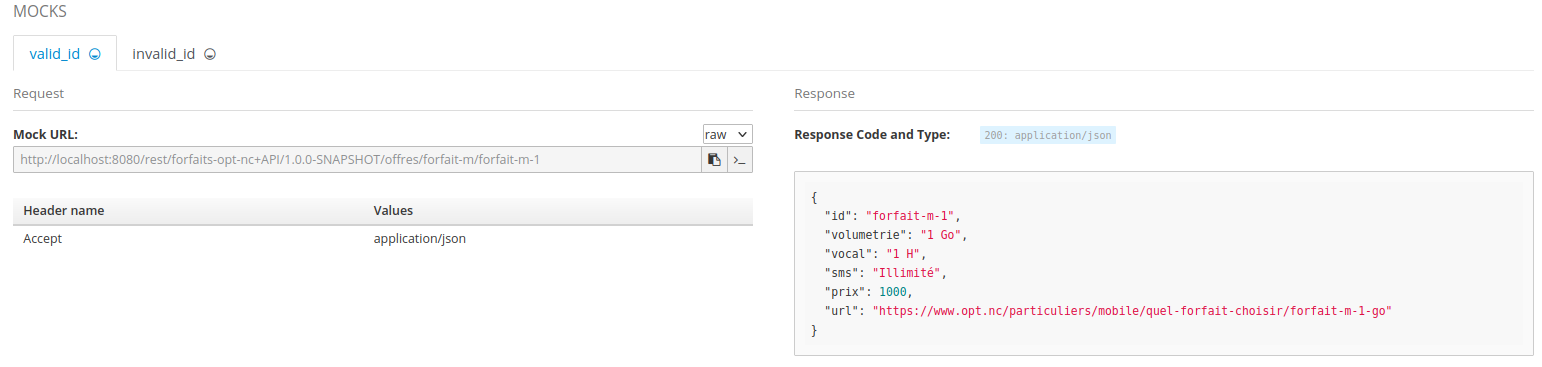
\includegraphics[width=\textwidth]{asset/mock_forfaitm.png}
			\caption{Endpoint \texttt{/offres/forfait-m/\{id\}} dans Microcks avec paramètre valide}
			\label{fig:endpoint-offres/forfait-m/{id}}
		\end{figure}
		
		Tandis qu'ici l'exemple est fait avec un paramètre invalide :
		
			\begin{figure}[H]
			\centering
			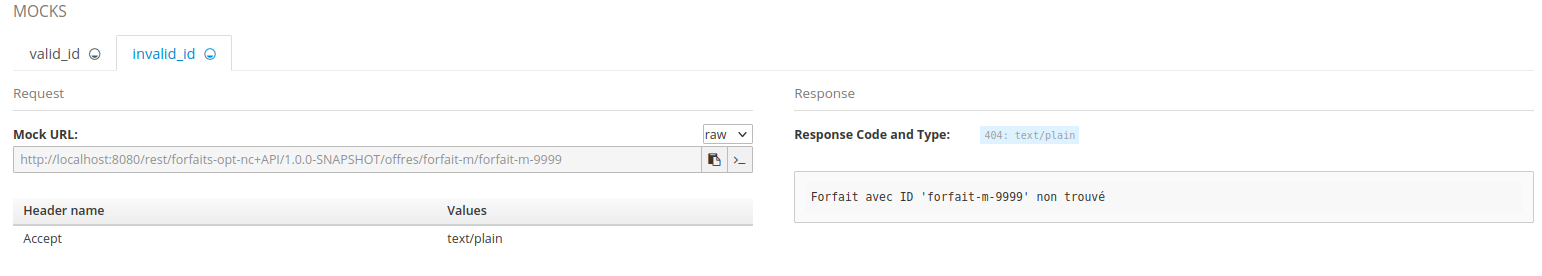
\includegraphics[width=\textwidth]{asset/microcks_invalid.png}
			\caption{Endpoint \texttt{/offres/forfait-m/{id}} dans Microcks avec paramètre invalide}
			\label{fig:endpoint-offres/forfait-m/{id}}
		\end{figure}
		
		Le \textbf{Conformance Index} de Microcks mesure à quel point les mocks sont conformes aux spécifications OpenAPI, est de \textbf{66.67\%}. Cela signifie que la simulation est proche à \textbf{66.67\%} du comportement attendu de l'API réelle.
		
		\begin{figure}[H]
			\centering
			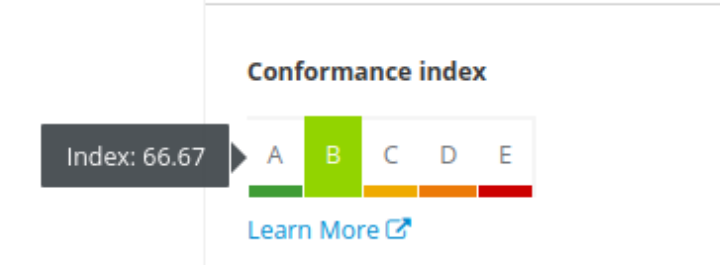
\includegraphics[width=0.5\textwidth]{asset/conformance-index.png}
			\caption{Conformance Index dans Microcks}
			\label{fig:conformance-index}
		\end{figure}
		
		\subsection*{Avantages de l'utilisation de Microcks}
		
		\begin{itemize}
			\item \textbf{Accessibilité pour les développeurs} : Si l'API n'est pas encore prête à être déployée, Microcks permet aux développeurs de tester l'API en simulant ses réponses, même si celle-ci n'est pas encore en production. Cela permet de continuer à avancer sur l'intégration sans attendre que l'API soit entièrement déployée.
			\item \textbf{Tests réalistes} : Grâce au conteneur Microcks, il est possible d'effectuer de vraies requêtes HTTP, offrant ainsi des tests réalistes
		\end{itemize}
		
		\section{From 0 to Hero}
		
		\subsection*{Acquisition de Compétences Techniques}
		
		Durant ce stage, j'ai significativement progressé dans différents domaines techniques et pratiques. Voici un tableau résumant mon évolution avant et après le stage, sur une échelle de 0 (aucune connaissance) à 5 (maîtrise avancée) :
		
		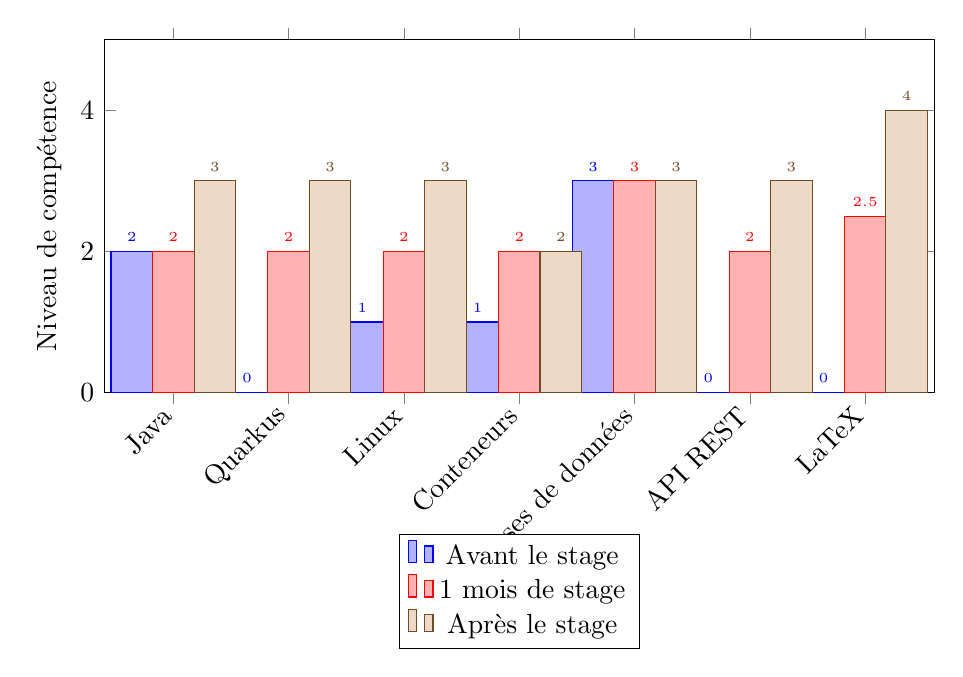
\begin{tikzpicture}
			\begin{axis}[
				ybar=0pt,
				bar width=15pt,
				symbolic x coords={Java, Quarkus,Linux, Conteneurs, Bases de données, API REST, LaTeX},
				xtick=data,
				x tick label style={rotate=45, anchor=east},
				ylabel={Niveau de compétence},
				xlabel={Compétences},
				legend style={at={(0.5,-0.4)}, anchor=north, legend columns=1}, % Légende beaucoup plus bas
				ymin=0,
				ymax=5,
				nodes near coords,
				every node near coord/.append style={font=\tiny},
				width=\textwidth,
				height=0.5\textwidth
				]
				% Données Avant le stage
				\addplot coordinates {(Java, 2) (Quarkus, 0) (Linux, 1) (Conteneurs, 1) (Bases de données, 3) (API REST, 0) (LaTeX, 0)};
				
				\addplot coordinates {(Java, 2) (Quarkus, 2) (Linux, 2) (Conteneurs, 2) (Bases de données, 3) (API REST, 2) (LaTeX, 2.5)};
	

				\addplot coordinates {(Java, 3) (Quarkus, 3) (Linux, 3) (Conteneurs, 2) (Bases de données, 3) (API REST, 3) (LaTeX, 4)};
				
				\legend{Avant le stage,1 mois de stage, Après le stage}
			\end{axis}
		\end{tikzpicture}
		
		\subsection*{Efforts et résultats}
		
		Au début du stage, mes compétences étaient limitées dans des domaines comme Quarkus, la conteneurisation et les APIs REST. Cependant, avec un travail régulier, j'ai rapidement progressé. L'intégration d'outils comme SonarQube et Microcks m'a permis d'améliorer la qualité du code et de comprendre l'importance de la CI/CD.
		
		\subsection*{Ressenti personnel}
		
			Ce stage a été une expérience très enrichissante, tant sur le plan technique que personnel. J'ai gagné en autonomie et appris à m'adapter à un environnement professionnel. Travailler sur un projet réel et en équipe, avec une bonne partie des travaux en remote et en pur cloud, m'a motivé et permis de renforcer ma confiance dans mes capacités à gérer des projets similaires à l'avenir.
		
	\section{Conclusion}
	
		Ce projet m'a permis de découvrir et d’aborder différentes facettes du développement d'une API, telles que l'intégration continue (CI), la gestion des migrations de base de données avec Flyway, la documentation automatique avec OpenAPI, Redocly et Bump.sh, ainsi que les tests unitaires et la couverture de code avec JaCoCo.
		
		\vspace{0.2cm}
		
		Grâce à ce stage, j’ai significativement progressé dans des domaines tels que le développement d'API, la conteneurisation et l’utilisation d’outils d'analyses et de documentation. J’ai aussi mieux compris l’importance de chaque étape dans la création d’une API, notamment pour améliorer la qualité du code et automatiser les processus avec des outils modernes.
		
		\vspace{0.2cm}
		
		Ce stage a été une véritable opportunité d’apprentissage, qui m’a préparé à de futurs défis professionnels et m’a donné une base solide pour continuer à évoluer dans le domaine du développement backend.


		
		\newpage
		\section{Annexe}
		\subsection{Illustrations}
			\begin{figure}[H]
			\centering
			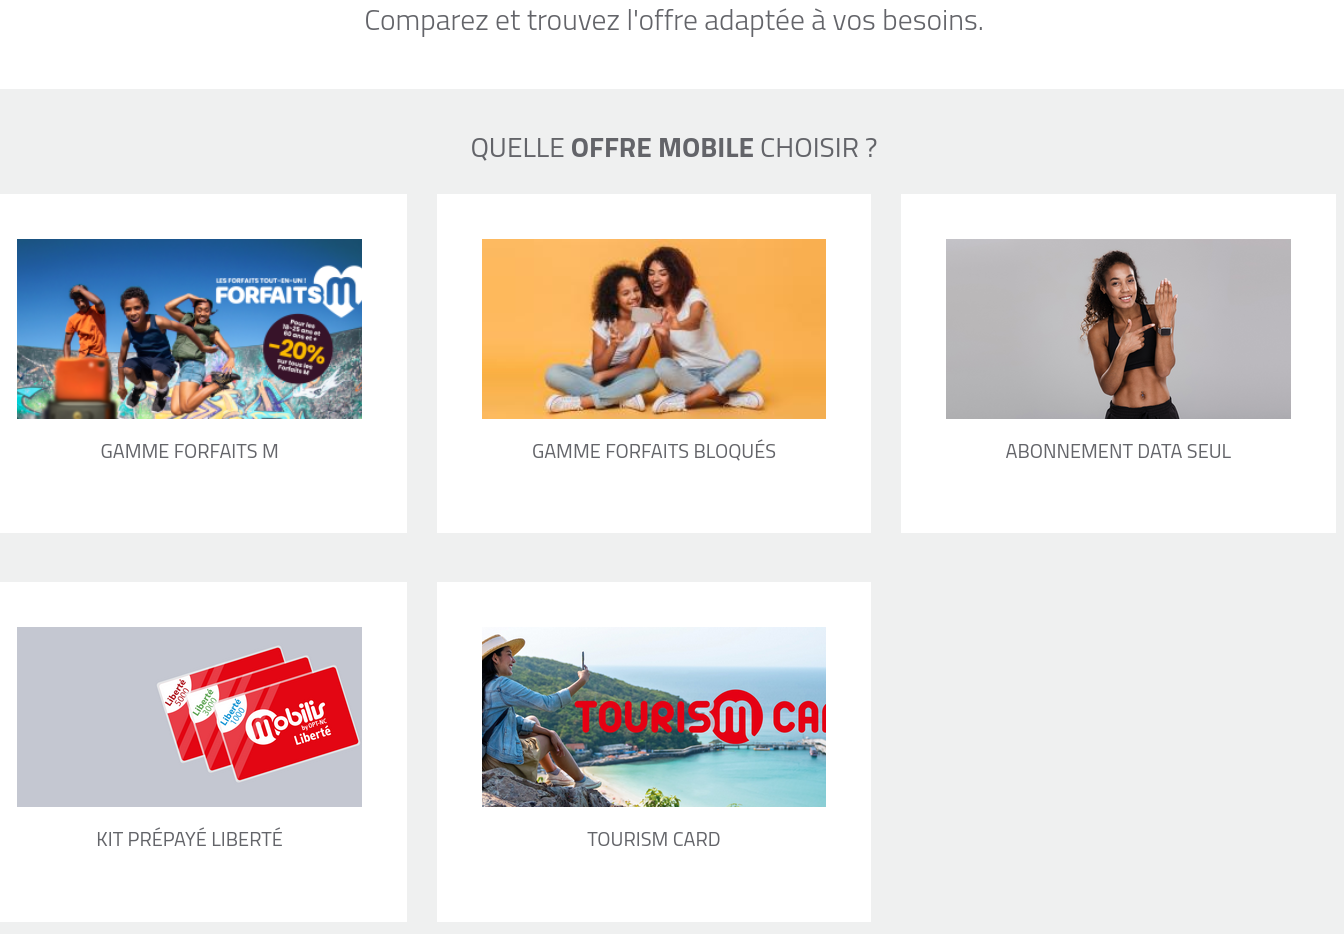
\includegraphics[width=0.8\textwidth]{asset/page_forfait.png}
			\caption{Page \textit{"Identifiez le forfait qui vous ressemble"} sur le site de l’OPT.}
			\label{fig:page_forfait}
		\end{figure}
		\begin{figure}[H]
			\centering
			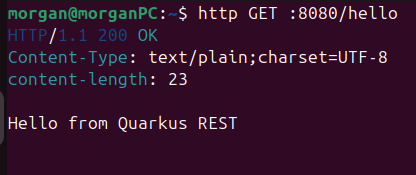
\includegraphics[width=0.8\textwidth]{asset/hello.png}
			\caption{Test de l'endpoint \texttt{/hello} avec HTTPIE.}
			\label{fig:hello_endpoint}
		\end{figure}
		\begin{figure}[H]
			\centering
			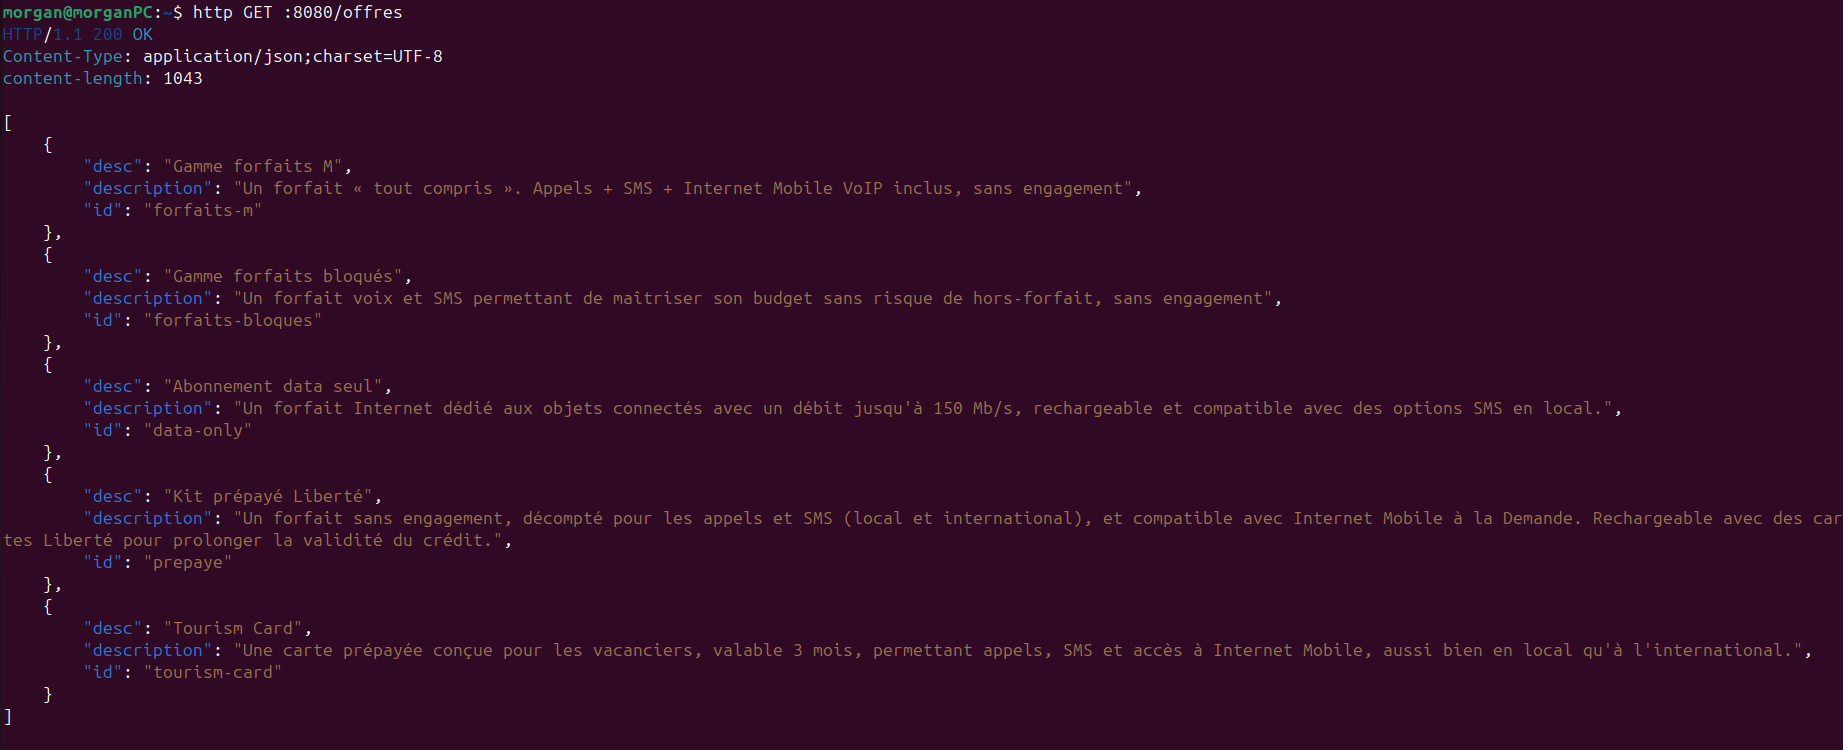
\includegraphics[width=1\textwidth]{asset/endpoint offres.png}
			\caption{Validation de l'endpoint \texttt{/offres} avec HTTPIE.}
			\label{fig:offres_endpoint}
		\end{figure}
		\begin{figure}[H]
			\centering
			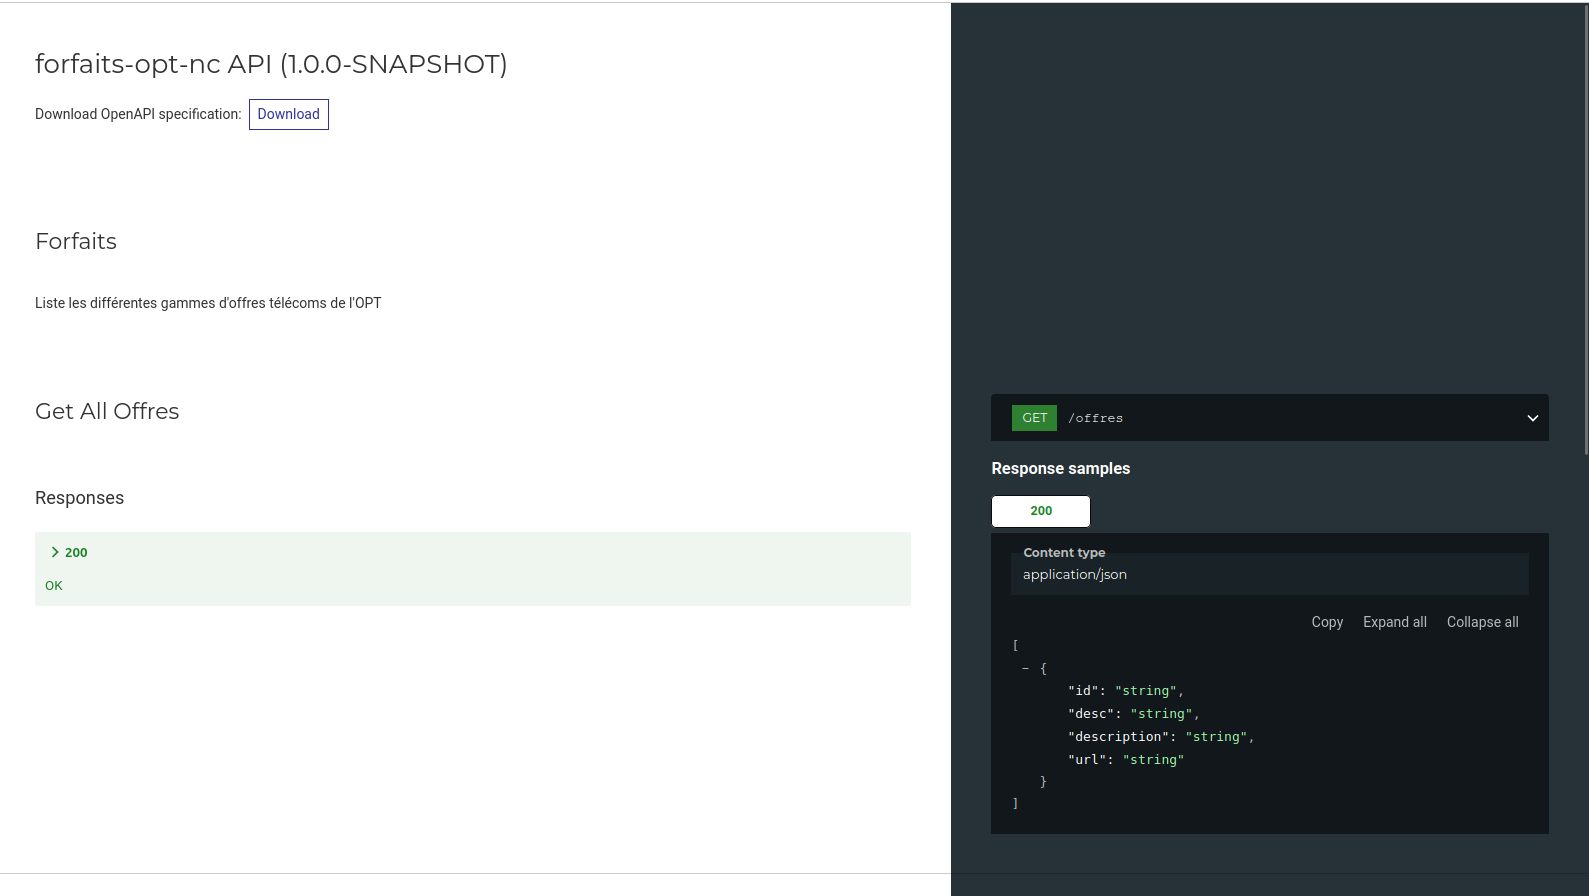
\includegraphics[width=\textwidth]{asset/redocly.png}
			\caption{Capture d'écran de la documentation Redocly}
			\label{fig:html_redocly}
		\end{figure}
		\begin{figure}[H]
			\centering
			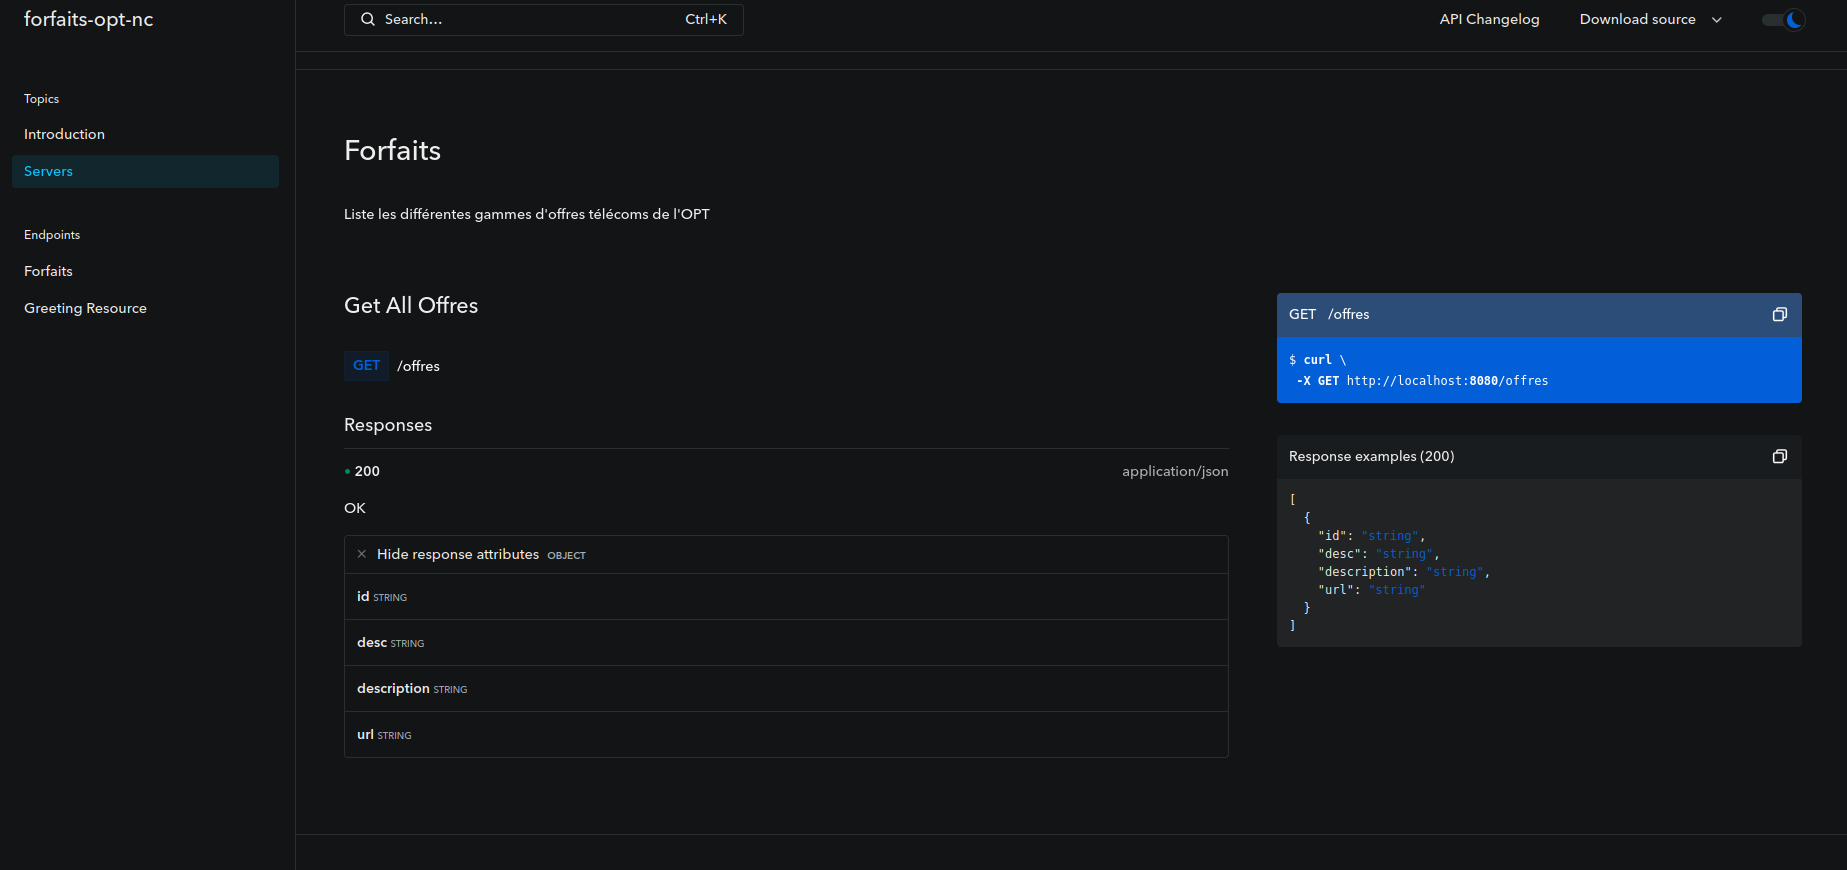
\includegraphics[width=\textwidth]{asset/bump-sh-documentation.png}
			\caption{Capture d'écran de la documentation générée par Bump.sh}
			\label{fig:bumpsh}
		\end{figure}
		\begin{figure}[H]
			\centering
			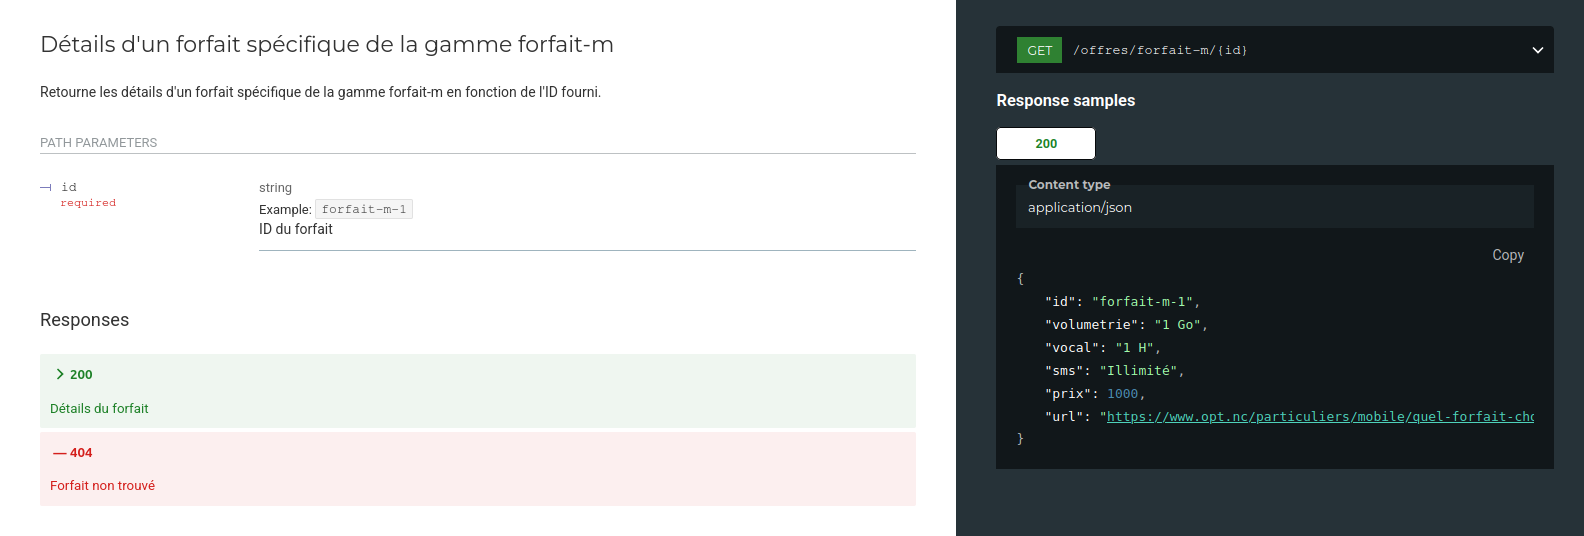
\includegraphics[width=\textwidth]{asset/Redocly_v2.png}
			\caption{Documentation générée par Redocly}
			\label{fig:redocly}
		\end{figure}
		\begin{figure}[H] \centering 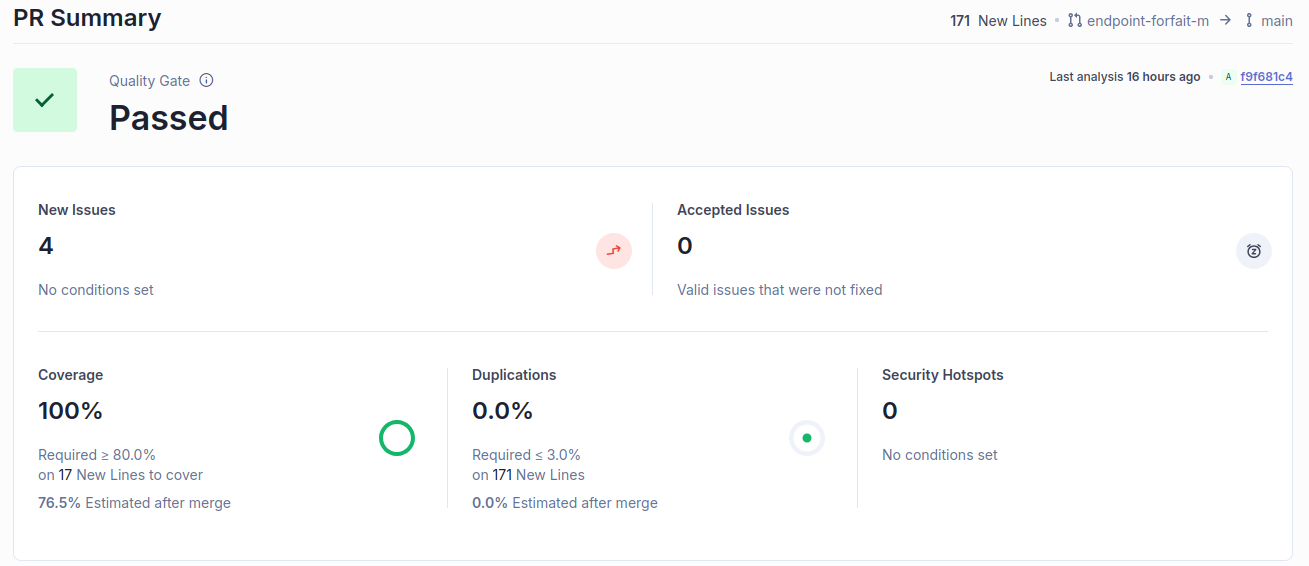
\includegraphics[width=\textwidth]{asset/analyse_sonarq.png} \caption{Analyse détaillée sur SonarQube} \label{fig:sonarq}\end{figure}
		\subsection{Bibliographie}
		\begin{itemize}
			\item \textbf{Documentation Quarkus} : Une ressource essentielle pour comprendre et utiliser Quarkus. Disponible sur : \url{https://quarkus.io/documentation/}
			\item \textbf{Documentation Flyway} : Guide pour utiliser Flyway dans Quarkus : \url{https://quarkus.io/guides/flyway}
			\item \textbf{Tutoriel sur HTTPie} : Introduction à l'utilisation de HTTPie pour tester des API REST. Disponible sur : \url{https://httpie.io/docs/cli}
			\item\textbf{Documentation Quarkus sur JIB} : \url{https://quarkus.io/guides/container-image#jib}
			\item \textbf{Podman Documentation} : Documentation officielle pour apprendre à gérer des conteneurs avec Podman. Disponible sur : \url{https://podman.io/documentation}
			\item \textbf{Tutoriel sur la génération de documentation statique avec OpenAPI et Redocly.} \url{https://redocly.com/docs/cli/} 
		\end{itemize}
		Articles du GLIA :
		\sloppy 
		\begin{itemize}
			\item \textbf{Annotations java :} \url{https://dev.to/optnc/openapi-java-annotation-for-better-\
				api-documentation-43oe}
			\item \textbf{Article sur OpenApi :} \url{https://dev.to/optnc/api-documentation-release-automation-with-github-redocly-and-open-api-f6h}
			\item \textbf{Build et déployer une documentation statique avec Quakus/Redocly sur Github Pages :} \url{https://dev.to/optnc/build-deliver-static-documentation-w-quarkusreodcly-on-github-pages-4224}
			\item \textbf {Site de bump.sh} : \url{https://bump.sh/}
			\item \textbf{Site SonarQube} : \url{https://www.sonarsource.com/products/sonarqube/}
			\item \textbf{Article sur Microcks par Vinh FAUCHER} : \url{https://dev.to/optnc/microcks-for-dummies-1imn}
			
		\end{itemize}
		
	\end{document}
